
\documentclass[a4paper,12pt]{scrbook}
\usepackage{amsmath,amssymb,amsthm}
\usepackage{fancyvrb}
\usepackage{parskip}
\usepackage{lastpage}
\usepackage{verbatim,boxedminipage,enumitem}
\usepackage{ifthen}
\usepackage{color,graphicx}
\usepackage{pgf}
\usepackage{longtable}
\usepackage{upquote}
%\usepackage[all]{xy}
\usepackage{tobiShell}
\usepackage{tikz}
\usetikzlibrary{automata}
\usetikzlibrary{arrows}
\usepackage{pgf,pgfarrows,pgfnodes}
\usepackage{pgfplots}
\usepackage{circuitikz}
\usetikzlibrary{circuits}
\usetikzlibrary{circuits.logic.US}
\usepackage{mymath}
\usepackage{python}
%------------------------------------------------------------------
% Verbatim for console window - single line frame, no line numbers
%------------------------------------------------------------------
\DefineVerbatimEnvironment%
 {console}{Verbatim}
 {frame=single}

%--------------------------------------------------------
% Remove the vertical spacing before and after Verbatim.
%--------------------------------------------------------
\usepackage{atbeginend}
\BeforeBegin{console}{\mbox{}\\ \begin{minipage}{\textwidth}\vspace{3pt}}
\AfterEnd{console}{\vspace{4pt} \end{minipage} \\ }

\begin{document}
\thispagestyle{empty}

\begin{center}
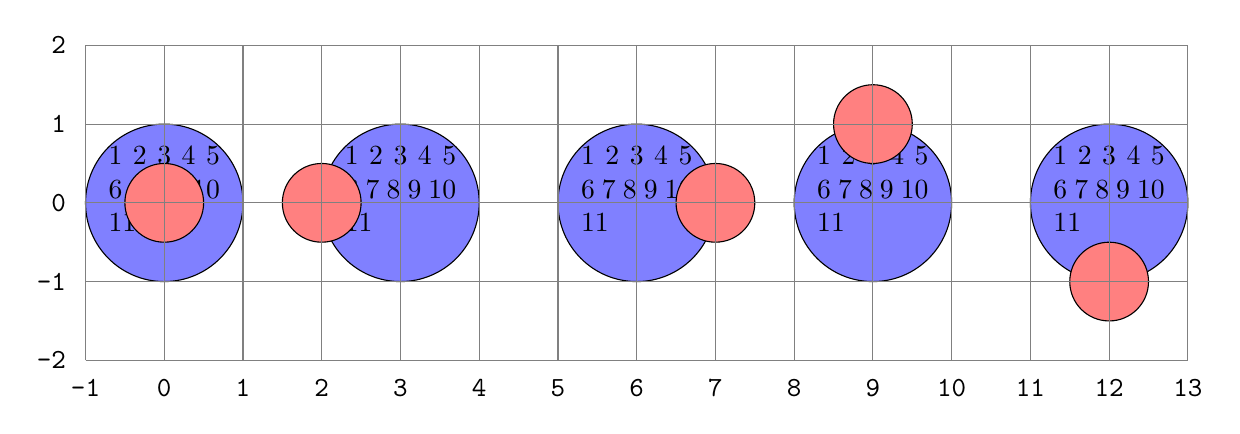
\begin{tikzpicture}
\fill[blue!50!white] (0.0, 0.0) circle (1);

\draw[black] (0.0, 0.0)
circle (1.0);

\draw (0.0,0.0) node[color=black, inner sep=0cm] {
 
\begin{minipage}[t][1.414cm]{1.414cm}
1 2 3 4 5 6 7 8 9 10 11
\end{minipage}

};\fill[red!50!white] (0.0, 0.0) circle (0.5);

\draw[black] (0.0, 0.0)
circle (0.5);
\fill[blue!50!white] (3.0, 0.0) circle (1);

\draw[black] (3.0, 0.0)
circle (1.0);

\draw (3.0,0.0) node[color=black, inner sep=0cm] {
 
\begin{minipage}[t][1.414cm]{1.414cm}
1 2 3 4 5 6 7 8 9 10 11
\end{minipage}

};\fill[red!50!white] (2.0, 0.0) circle (0.5);

\draw[black] (2.0, 0.0)
circle (0.5);
\fill[blue!50!white] (6.0, 0.0) circle (1);

\draw[black] (6.0, 0.0)
circle (1.0);

\draw (6.0,0.0) node[color=black, inner sep=0cm] {
 
\begin{minipage}[t][1.414cm]{1.414cm}
1 2 3 4 5 6 7 8 9 10 11
\end{minipage}

};\fill[red!50!white] (7.0, 0.0) circle (0.5);

\draw[black] (7.0, 0.0)
circle (0.5);
\fill[blue!50!white] (9.0, 0.0) circle (1);

\draw[black] (9.0, 0.0)
circle (1.0);

\draw (9.0,0.0) node[color=black, inner sep=0cm] {
 
\begin{minipage}[t][1.414cm]{1.414cm}
1 2 3 4 5 6 7 8 9 10 11
\end{minipage}

};\fill[red!50!white] (9.0, 1.0) circle (0.5);

\draw[black] (9.0, 1.0)
circle (0.5);
\fill[blue!50!white] (12.0, 0.0) circle (1);

\draw[black] (12.0, 0.0)
circle (1.0);

\draw (12.0,0.0) node[color=black, inner sep=0cm] {
 
\begin{minipage}[t][1.414cm]{1.414cm}
1 2 3 4 5 6 7 8 9 10 11
\end{minipage}

};\fill[red!50!white] (12.0, -1.0) circle (0.5);

\draw[black] (12.0, -1.0)
circle (0.5);
\draw[gray] (-1.0,-2.0) -- (-1.0,2);
\draw[gray] (0.0,-2.0) -- (0.0,2);
\draw[gray] (1.0,-2.0) -- (1.0,2);
\draw[gray] (2.0,-2.0) -- (2.0,2);
\draw[gray] (3.0,-2.0) -- (3.0,2);
\draw[gray] (4.0,-2.0) -- (4.0,2);
\draw[gray] (5.0,-2.0) -- (5.0,2);
\draw[gray] (6.0,-2.0) -- (6.0,2);
\draw[gray] (7.0,-2.0) -- (7.0,2);
\draw[gray] (8.0,-2.0) -- (8.0,2);
\draw[gray] (9.0,-2.0) -- (9.0,2);
\draw[gray] (10.0,-2.0) -- (10.0,2);
\draw[gray] (11.0,-2.0) -- (11.0,2);
\draw[gray] (12.0,-2.0) -- (12.0,2);
\draw[gray] (13.0,-2.0) -- (13.0,2);
\draw[gray] (-1.0,-2.0) -- (13,-2.0);
\draw[gray] (-1.0,-1.0) -- (13,-1.0);
\draw[gray] (-1.0,0.0) -- (13,0.0);
\draw[gray] (-1.0,1.0) -- (13,1.0);
\draw[gray] (-1.0,2.0) -- (13,2.0);
\draw(-1, -2) node [font=\ttfamily, label=below:{\texttt{-1}}] {};
\draw(0, -2) node [font=\ttfamily, label=below:{\texttt{0}}] {};
\draw(1, -2) node [font=\ttfamily, label=below:{\texttt{1}}] {};
\draw(2, -2) node [font=\ttfamily, label=below:{\texttt{2}}] {};
\draw(3, -2) node [font=\ttfamily, label=below:{\texttt{3}}] {};
\draw(4, -2) node [font=\ttfamily, label=below:{\texttt{4}}] {};
\draw(5, -2) node [font=\ttfamily, label=below:{\texttt{5}}] {};
\draw(6, -2) node [font=\ttfamily, label=below:{\texttt{6}}] {};
\draw(7, -2) node [font=\ttfamily, label=below:{\texttt{7}}] {};
\draw(8, -2) node [font=\ttfamily, label=below:{\texttt{8}}] {};
\draw(9, -2) node [font=\ttfamily, label=below:{\texttt{9}}] {};
\draw(10, -2) node [font=\ttfamily, label=below:{\texttt{10}}] {};
\draw(11, -2) node [font=\ttfamily, label=below:{\texttt{11}}] {};
\draw(12, -2) node [font=\ttfamily, label=below:{\texttt{12}}] {};
\draw(13, -2) node [font=\ttfamily, label=below:{\texttt{13}}] {};
\draw(-1, -2) node [font=\ttfamily, label=left:{\texttt{-2}}] {};
\draw(-1, -1) node [font=\ttfamily, label=left:{\texttt{-1}}] {};
\draw(-1, 0) node [font=\ttfamily, label=left:{\texttt{0}}] {};
\draw(-1, 1) node [font=\ttfamily, label=left:{\texttt{1}}] {};
\draw(-1, 2) node [font=\ttfamily, label=left:{\texttt{2}}] {};
\end{tikzpicture}

\end{center}

\end{document}
